Solution times reported are from an Intel Core i5-4288U @ 2.6 GHz running macOS Catalina. Simulations showed that \texttt{HPIPM} is significantly faster in solving the partially condensed QP arising in the NMPC formulation than the corresponding dense QP. The average times per SQP-iteration in \texttt{acados} were $4.27$ ms for the novice and $3.87$ ms for the experienced pilot. It is interesting to note that one can modify $N_b$ and potentially improve the blending mechanism performance without affecting solution times significantly. Fig.~\ref{fig:violin} shows that all quantities appear to be related to $N$ rather than $N_b$.

As previously mentioned, partial condensing is an approach in-between the sparse and the condensed one. Here, in particular, the horizon length can be reduced at the expense of a larger input vector. This degree of freedom is used to find the best subproblem size for \texttt{HPIPM}. Thus, given the dimensions of the resulting QP subproblems in our controller, computational efficiency is granted through partial condensing as it allows us to exploit hardware throughput better.

\begin{figure}[t]
	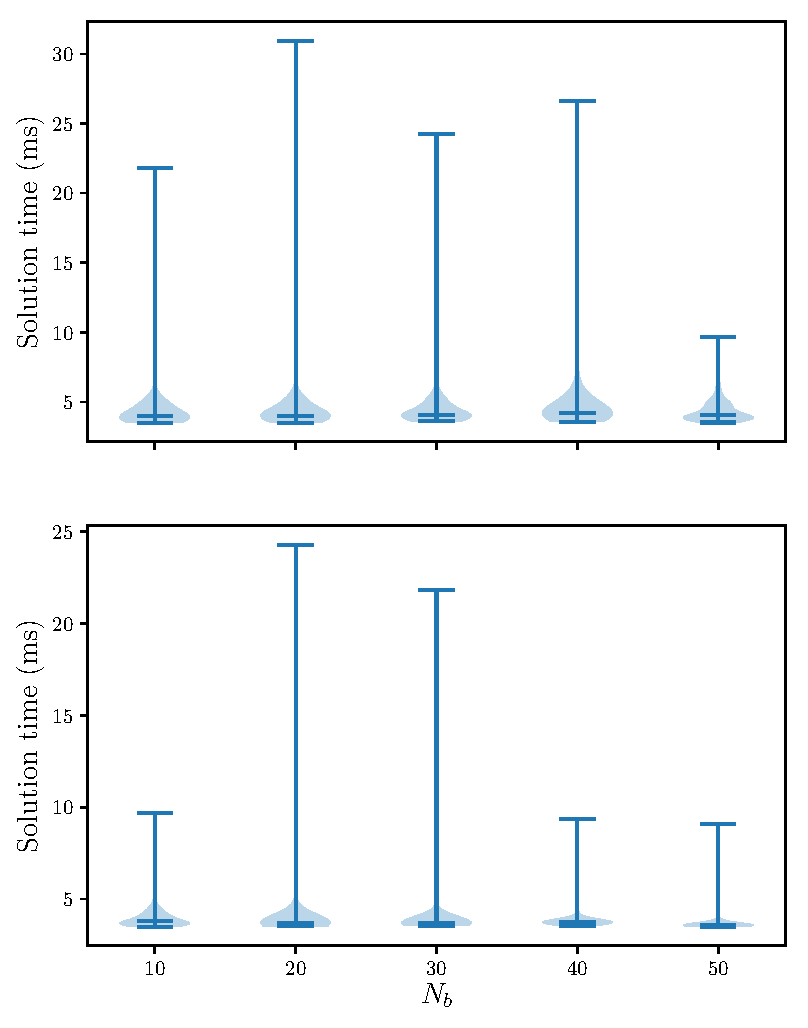
\includegraphics[width=0.5\textwidth]{figures/violin}
	\vspace{-0.8cm}
	\caption{Violin plot representations of the solution times associated with the mixed-initiative controller in simulations with a novice (top) and an experienced pilot (bottom). Central bars represent the median values for each virtual horizon $N_b$.}\label{fig:violin}
\end{figure}